\documentclass[runningheads]{llncs}
\usepackage{graphicx}
\usepackage{amsmath,amssymb} % define this before the line numbering.
\usepackage{color}
\usepackage[width=122mm,left=12mm,paperwidth=146mm,height=193mm,top=12mm,paperheight=217mm]{geometry}
%\usepackage{ruler}
\usepackage{url}

\begin{document}
\newcommand{\todo}[1]{{\color{red} {\bf TODO:} \it #1}}
\newcommand{\ning}[1]{{\color{blue}{\bf Ning:} \it #1}}
\renewcommand{\tabcolsep}{0.2cm}

\pagestyle{headings}
\mainmatter
%\def\ECCV14SubNumber{1074}  % Insert your submission number here

\title{Part-based R-CNNs for \\ Fine-grained Category Detection}

\titlerunning{Part-based R-CNNs for Fine-grained Category Detection}

\authorrunning{Zhang, Donahue, Girshick, Darrell}

\author{Ning Zhang, Jeff Donahue, Ross Girshick, Trevor Darrell\\
\texttt{\{nzhang,jdonahue,rbg,trevor\}@eecs.berkeley.edu}}
\institute{University of California, Berkeley}

\maketitle

\begin{abstract}
\begin{abstract}

We propose a convolutional neural network (CNN) architecture for facial expression recognition. The proposed architecture is independent of any hand-crafted feature extraction and performs better than the earlier proposed convolutional neural network based approaches. We visualize the automatically extracted features which have been learned by the network in order to provide a better understanding. The standard datasets, i.e. Extended Cohn-Kanade (CKP) and MMI Facial Expression Databse are used for the quantitative evaluation. On the CKP set the current state of the art approach, using CNNs, achieves an accuracy of 99.2\%. For the MMI dataset, currently the best accuracy for emotion recognition is 93.33\%. The proposed architecture achieves $99.6$\% for CKP and $98.63$\% for MMI, therefore performing better than the state of the art using CNNs. Automatic facial expression recognition has a broad spectrum of applications such as human-computer interaction and safety systems. This is due to the fact that non-verbal cues are important forms of communication and play a pivotal role in interpersonal communication. The performance of the proposed architecture endorses the efficacy and reliable usage of the proposed work for real world applications.

\end{abstract}

\keywords{Fine-grained recognition, object detection, convolutional models}
\end{abstract}


%\cite{burger2001issues}
%\cite{fader2014open}
%\cite{voorhees1999trec}


%A huge leap forward in artificial intelligence will be achieved when
%machines will be able to answer any question expressed in natural
%language. As such, q

Question answering (QA) has been a long standing research problem in
natural language processing, with the first systems attempting to
answer questions by directly reading
documents \citep{voorhees2000building}. The development of large-scale Knowledge Bases (KBs) such as Freebase  \citep{bollacker2008freebase}
helped organize information into structured forms, prompting recent progress to focus on answering questions by converting them into logical forms that can be used to query such databases \citep{berant2013semantic,kwiatkowski-EtAl:2013:EMNLP,fader2014open}.

Unfortunately, KBs have intrinsic limitations such as their inevitable incompleteness and fixed schemas that cannot support all varieties of answers.
%
Since information extraction (IE) \citep{craven2000learning}, intended to
fill in missing information in KBs, is neither accurate nor
reliable enough, collections of raw textual resources and
documents such as Wikipedia will always contain more information.
%than KBs.
%
As a result, even if KBs can be satisfactory for closed-domain problems, they are unlikely
to scale up to answer general questions on any
topic.
%
Starting from this observation,
%here we propose  to study the problem
in this work we study the problem
of answering by directly reading documents.


Retrieving answers directly from text is harder than
from KBs because information is far less structured, is
indirectly and ambiguously expressed, and is usually scattered across multiple documents.
%
%This explains why, when a satisfactory KB is
%available -- which is typically only the case in closed domains --
%using it instead of raw text is preferred. %, because performance is better.
%
This explains why using a satisfactory KB---typically only available in closed domains---is preferred over raw text.
%
We postulate that before trying to provide answers that are not in
KBs, document-based QA systems should first reach KB-based systems'
performance in such closed domains, where clear comparison and
evaluation is possible.
%
To this end, this paper introduces {\sc WikiMovies}, a new
analysis tool that allows for measuring the performance of %loss induced on
QA systems when the knowledge source is switched from a KB to unstructured documents.
%
{\sc WikiMovies} contains $\sim$100k questions in the movie domain, and was designed
to be answerable by using either a perfect KB
(based on OMDb\footnote{\url{http://www.omdbapi.com}}), Wikipedia pages or an imperfect KB obtained through
running %a standard IE pipeline on those pages.
an engineered IE pipeline on those pages.

To bridge the gap between using a KB and reading documents directly,
we still lack appropriate machine learning algorithms. In this
work we propose the Key-Value Memory Network (KV-MemNN), a new neural network
architecture that generalizes the original Memory Network
\citep{sukhbaatar2015end} and can work with either knowledge source.
%
The KV-MemNN performs QA by first storing facts in a key-value
structured memory before reasoning on them in order to predict an
answer. The memory is designed so that the model learns to use keys to
address relevant memories with respect to the question, whose corresponding values are subsequently returned.
%
This structure allows the model to encode prior knowledge for the considered task
and to leverage possibly complex transforms between keys and values,
while still being trained using standard backpropagation via
stochastic gradient descent.

Our experiments on {\sc WikiMovies} indicate that, thanks to its key-value memory,
the KV-MemNN consistently outperforms the
original Memory Network, and reduces the gap between answering from a human-annotated KB,
from an automatically extracted KB or from directly reading Wikipedia.
%
We confirm our findings on  {\sc WikiQA} \citep{yang2015wikiqa},
another Wikipedia-based QA benchmark where no KB is available,
where we demonstrate that KV-MemNN can reach state-of-the-art results---surpassing
the most recent attention-based neural network models.


The majority of existing approaches to WSD formulate this task as  MIL. In this formulation an image is interpreted as a bag of regions. If the image is labeled as positive, then one of the regions is assume to tightly contain the object of interest. If the image is labeled as negative, then no region contains the object. Learning alternates between estimating a model of the object appearance and selecting which regions in the positive bags correspond to the object using the appearance model. 

The MIL strategy results in a non-convex optimization problem; in practice, solvers tend to get stuck in local optima such that the quality of the solution strongly depends on the initialization. Several papers have focused on developing various initialization strategies \cite{Kumar10a,Deselaers10,Song14a,Cinbis15} and on regularizing the optimization problem \cite{Song14,Bilen14}. Kumar~\etal \cite{Kumar10a} propose a self-paced learning strategy that progressively includes harder samples to a small set of initial ones at training. Deselaers~\etal~\cite{Deselaers10} initialize object locations based on the objectness score. Cinbis~\etal \cite{Cinbis15} propose a multi-fold split of the training data to escape local optima. Song~\etal~\cite{Song14} apply Nesterov's smoothing technique \cite{Nesterov05} to the latent SVM formulation \cite{Felzenszwalb10a} to be more robust against poor initializations. Bilen~\etal~\cite{Bilen14} propose a smoothed version of MIL that softly labels object instances instead of choosing the highest scoring ones. Additionally, their method regularizes the latent object locations by penalizing unlikely configurations based on symmetry and mutual exclusion principles.

Another line of research in WSD \cite{Song14,Song14a,Wang14a} is based on the idea of identifying the similarity between image parts. Song~\etal \cite{Song14} propose a discriminative graph-based algorithm that selects a subset of windows such that each window is connected to its nearest neighbors in positive images. In~\cite{Song14a}, the same authors extend this method to discover multiple co-occurring part configurations. Wang~\etal~\cite{Wang14a} propose an iterative technique that applies a latent semantic clustering via latent Semantic Analysis (pLSA) on the windows of positive samples and selects the most discriminative cluster for each class based on its classification performance. Bilen~\etal \cite{Bilen15} propose a formulation that jointly learns a discriminative model and enforces the similarity of the selected object regions via a discriminative convex clustering algorithm.

Recently a number of researchers \cite{Oquab14,Oquab15} have proposed weakly supervised localization principles to improve classification performance of CNNs without providing any annotation for the location of objects in images. Oquab~\etal \cite{Oquab14} employ a pre-trained CNN to compute a mid-level image representation for images of PASCAL VOC. In their follow-up work, Oquab~\etal \cite{Oquab15} modify a CNN architecture to \emph{coarsely} localize object instances in image while predicting its label. 

Jaderberg~\etal~\cite{Jaderberg15c} proposed a CNN architecture in which a subnetwork automatically pre-transforms an image in order to optimize the classification accuracy of a second subnetwork. This ``transformer network'', which is trained in an end-to-end fashion from image-level labels, is shown to align objects to a common reference frame, which is a proxy to detection. Our architecture contains a mechanism that pre-select image regions that are likely to contain the object, also trained in an end-to-end fashion; while this may seem very different, this mechanism can also be thought as learning transformations (as the ones that map the detected regions to a canonical reference frame). However, the nature of the selection process in in our and their networks are very different.


\begin{figure*}
\centering
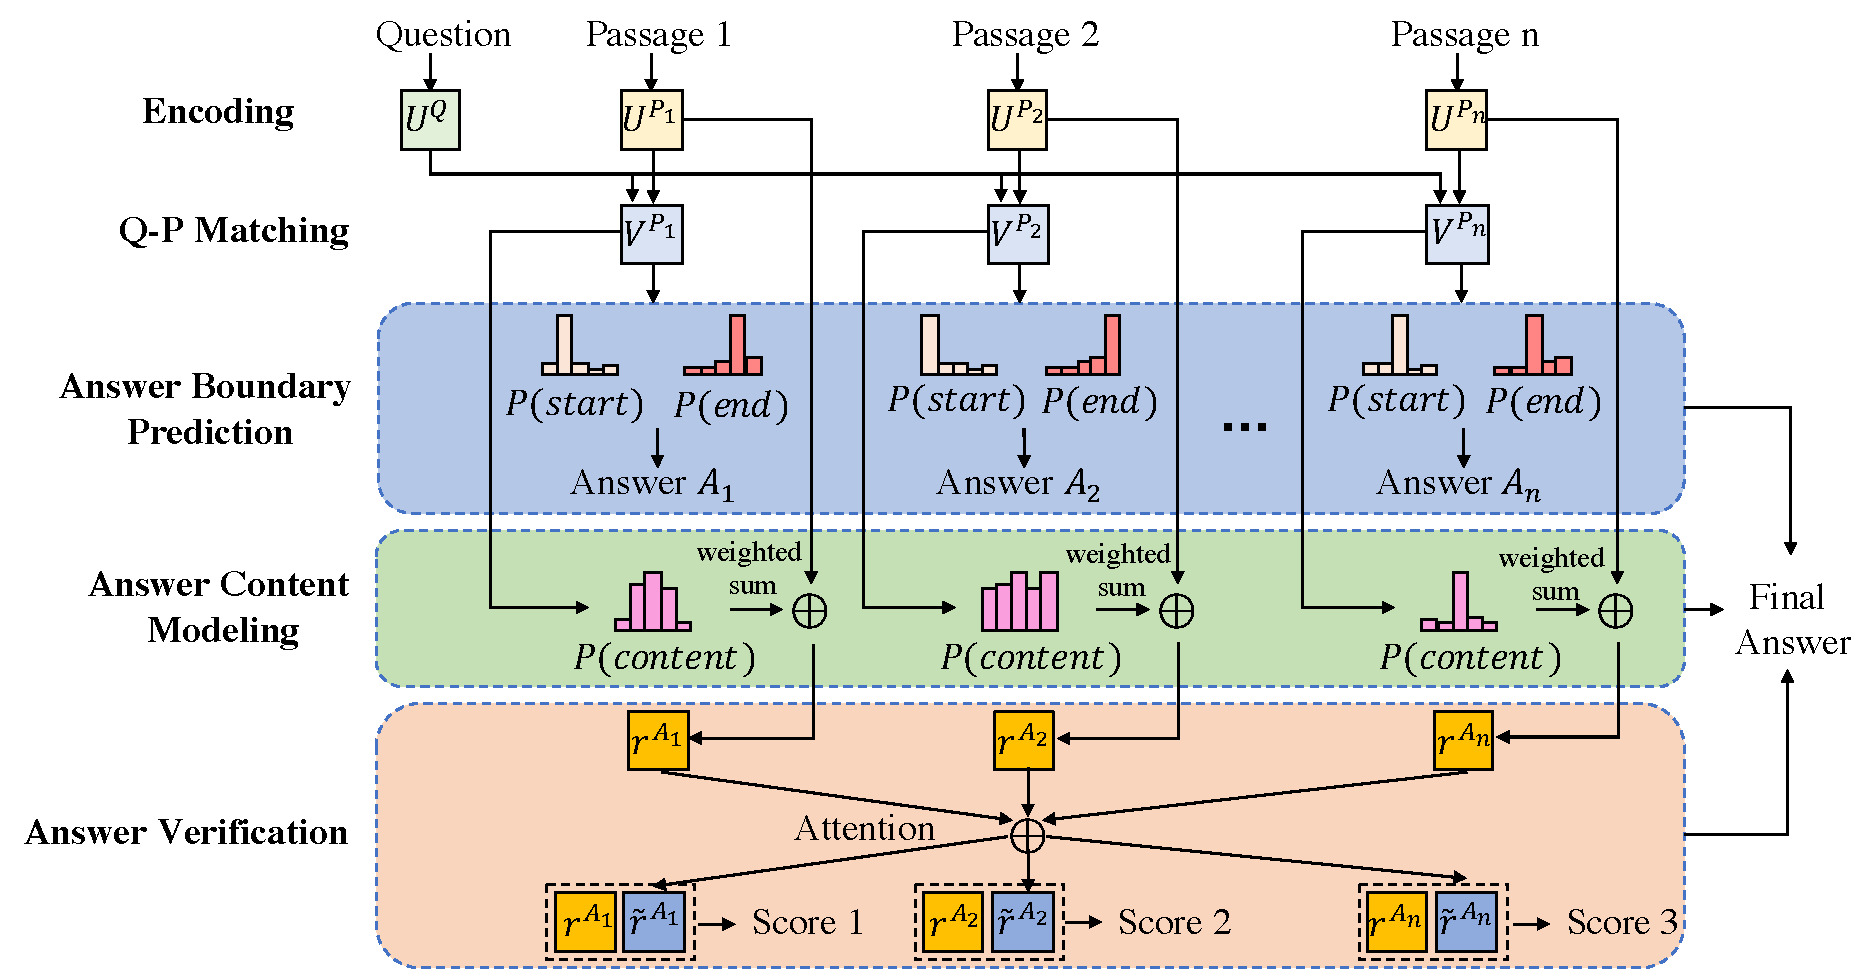
\includegraphics[width=0.85\textwidth]{architecture}
\caption{The overall architecture of our proposed network. The network
contains layers of symmetric convolution (encoder) and deconvolution (decoder).
Skip shortcuts are connected every a few (in our experiments, two) layers from
convolutional feature maps to their mirrored deconvolutional feature maps.
The response from a convolutional layer is directly propagated to the corresponding
mirrored deconvolutional layer, both forwardly and backwardly.}
\label{fig1}
\end{figure*}

\section{Very deep convolutional auto-encoder for image restoration}
\label{sec:main}

The proposed framework mainly contains a chain of convolutional layers and symmetric
deconvolutional layers, as shown in Figure \ref{fig1}. Skip connections are connected
symmetrically from convolutional layers to deconvolutional layers. We term our method
``RED-Net''---very deep Residual Encoder-Decoder Networks.


\subsection{Architecture}

The framework is fully convolutional (and deconvolutional.  Deconvolution is essentially unsampling convolution). Rectification layers are added
after each convolution and deconvolution. For low-level image restoration problems, we
use neither pooling nor unpooling in the network as usually pooling discards useful image
details that are essential for these tasks. It is worth mentioning that since the convolutional
and deconvolutional layers are symmetric, the network is essentially pixel-wise prediction,
thus the size of input image can be arbitrary. The input and output of the network are images
of the same size $w\times h\times c$, where $w$, $h$ and $c$ are width, height and number of channels.

Our main idea is that the convolutional layers act as a feature extractor, which preserve the
primary components of objects in the image and meanwhile eliminating the corruptions.
After forwarding through the convolutional layers, the corrupted input  image is converted into
a ``clean" one. The subtle details of the image contents may be lost during this process.
The deconvolutional layers are then combined to recover the details of image contents.
The output of the deconvolutional layers is the recovered clean version of the input image.
Moreover, we add skip connections  from a convolutional layer to its corresponding
mirrored deconvolutional layer. The passed convolutional feature maps are summed to the
deconvolutional feature maps element-wise, and passed to the next layer after rectification.
Deriving from the above architecture, we have used two networksvin our experiments, which are of 20 layers
 and 30 layers
respectively, for image denoising, image super-resolution, JPEG deblocking and image inpainting.



\subsection{Deconvolution decoder}

Architectures combining layers of convolution and deconvolution~\cite{DBLP:conf/iccv/NohHH15,
hong2015decoupled} have been proposed for semantic segmentation recently. In contrast to
convolutional layers, in which multiple input activations within a filter window are fused
to output a single activation, deconvolutional layers associate a single input activation with
multiple outputs. Deconvolution is usually used as {\em learnable up-sampling layers}.

 In our network,
the convolutional layers successively down-sample the input image content into a  small
size abstraction. Deconvolutional layers then up-sample the abstraction back into its original resolution.

Besides the use of skip connections, a main difference between our model and
~\cite{DBLP:conf/iccv/NohHH15,hong2015decoupled} is that our network is fully convolutional and
deconvolutional, i.e., without pooling and un-pooling. The reason is that for low-level image restoration,
the aim is to eliminate low level corruption while preserving image details instead of learning
image abstractions. Different from high-level applications such as segmentation or recognition,
pooling typically eliminates the abundant image details and can deteriorate restoration performance.



One can simply replace deconvolution with convolution, which results in an architecture that is
very similar to recently proposed very deep fully convolutional neural networks
~\cite{DBLP:conf/cvpr/LongSD15,DBLP:journals/pami/DongLHT16}. However, there exist essential
differences between a fully convolution model and our model. Take image denoising as an example.
We compare the 5-layer and 10-layer fully convolutional network with our network
(combining convolution and deconvolution, but without skip connection). For fully convolutional
networks, we use padding or up-sampling the input to make the input and output be of the same size.
For our network, the first 5 layers are convolutional and the second 5 layers are deconvolutional.
All the other parameters for training are identical, i.e., trained with SGD and learning rate of
$10^{-6}$, noise level $\sigma=70$. The Peak Signal-to-Noise Ratio (PSNR) on the validation set
is reported, which shows that using deconvolution works better than the fully convolutional
counterpart, as shown in Figure \ref{fig2}.


Furthermore, in Figure \ref{fig3}, we visualize some results that are outputs of layer 2, 5, 8 and 10
from the 10-layer fully convolutional network and ours. In the fully convolution case, the noise
is eliminated step by step, i.e., the noise level is reduced after each layer. During this process,
the details of the image content may be lost. Nevertheless, in our network, convolution  preserves
the primary image content. Then deconvolution is used to compensate the details.


\begin{figure}[htb!]
\centering
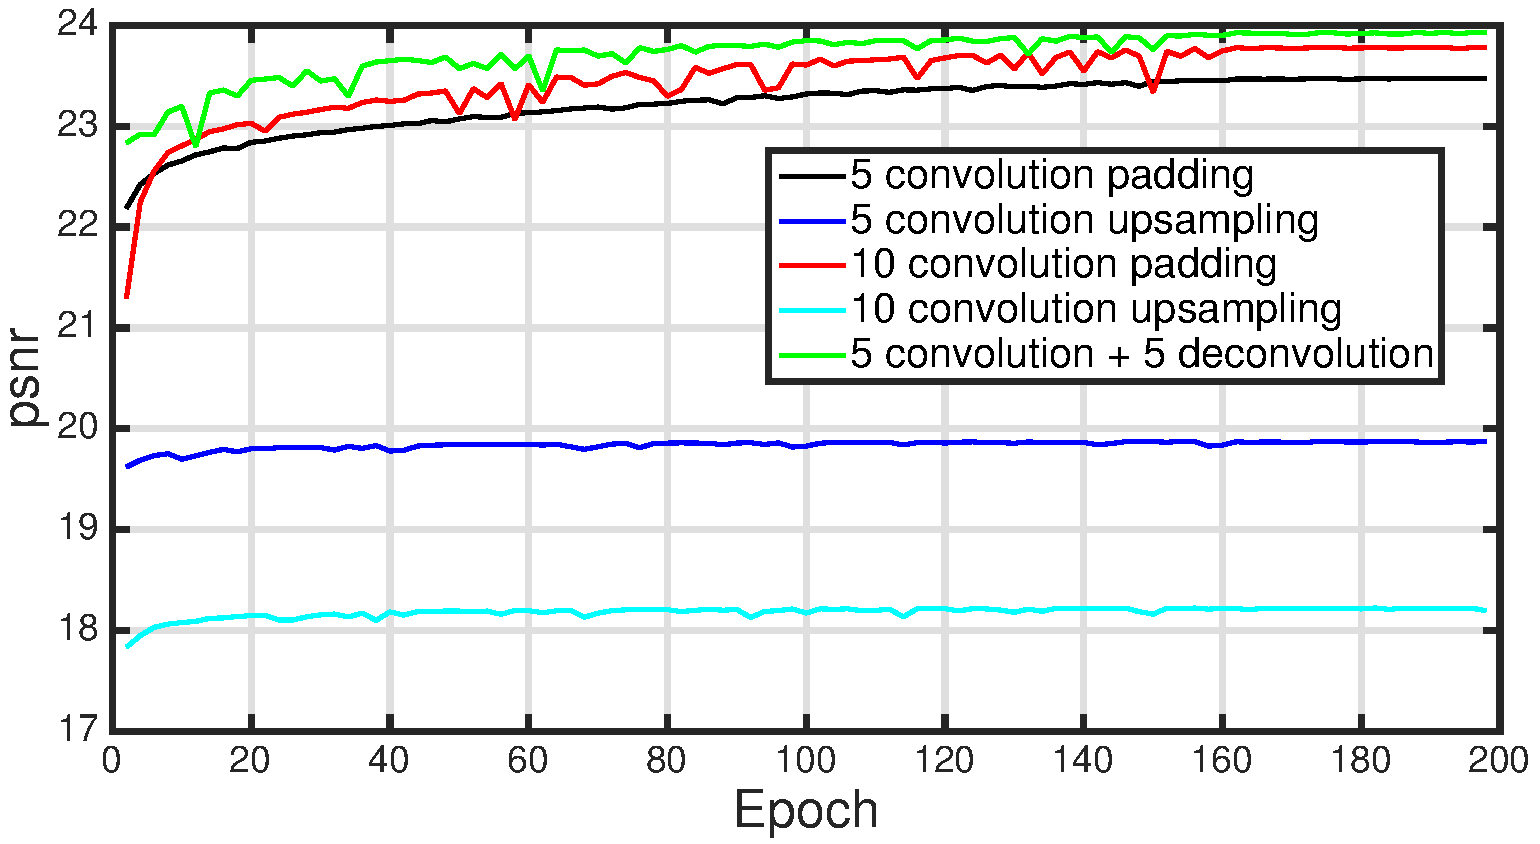
\includegraphics[width=0.48\textwidth]{conv-vs-decv}
\caption{ PSNR  values  on the validation set during training. Our model  exhibits better PSNR
than the compared ones upon convergence.}
\label{fig2}
\end{figure}



\begin{figure}[htb!]
\centering
\subfigure[]{ 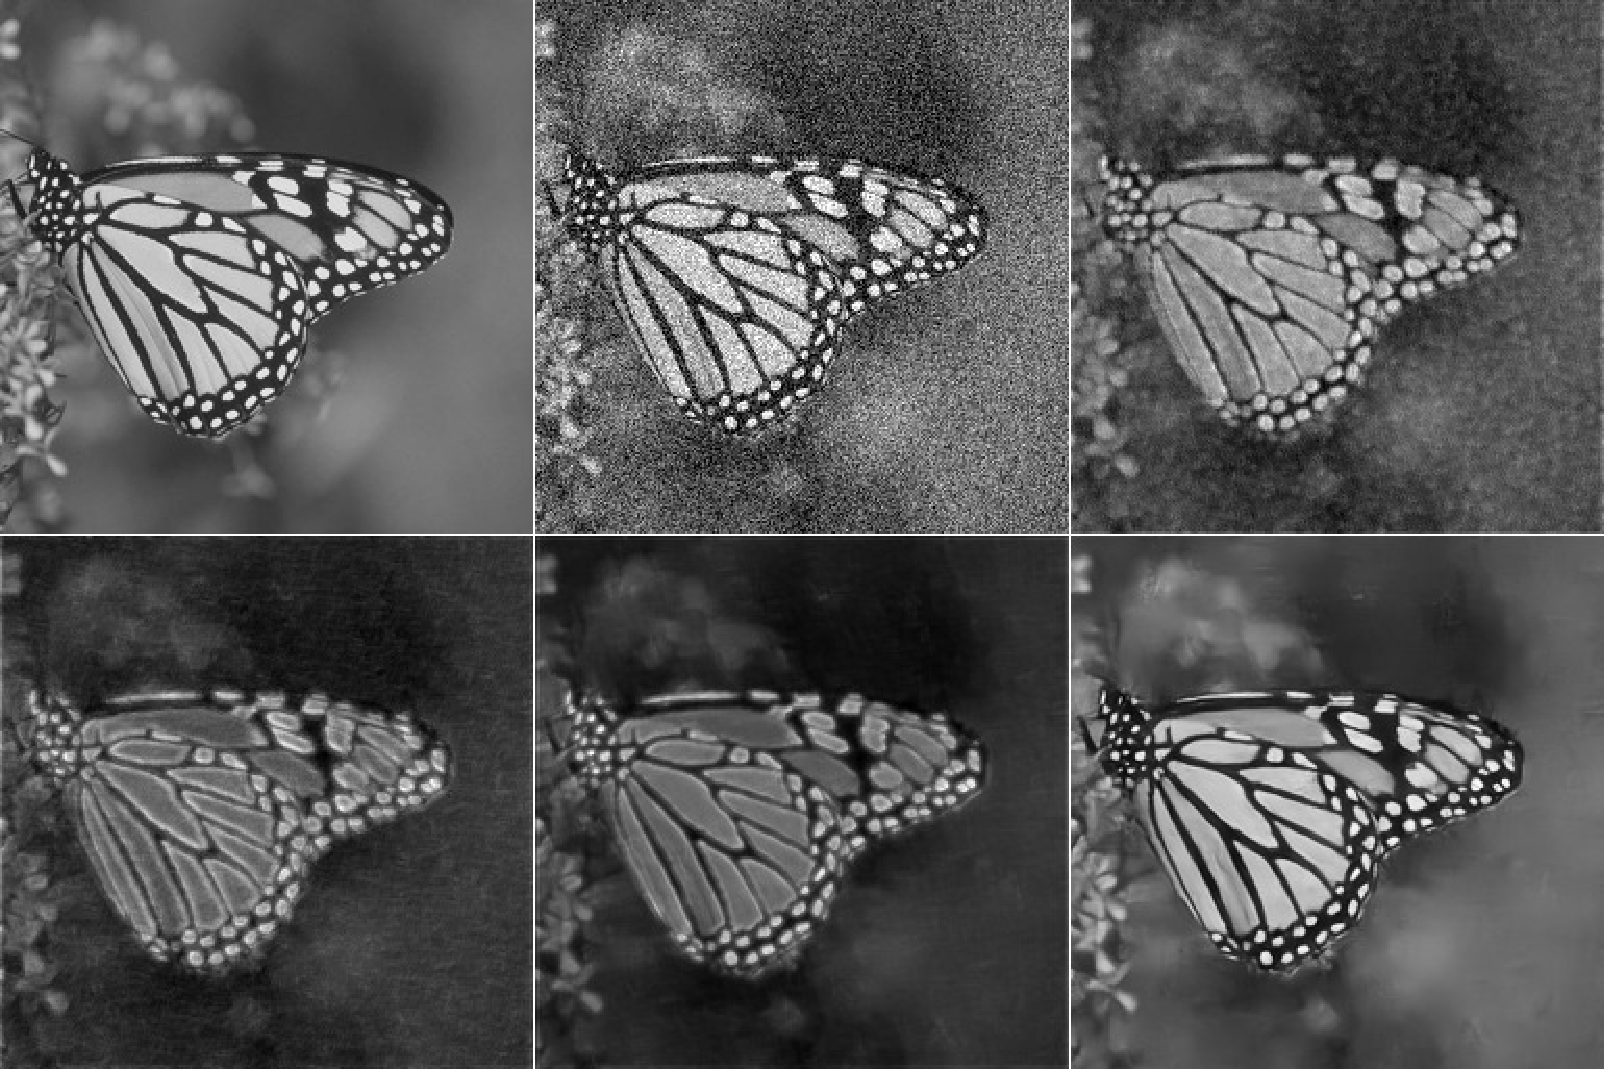
\includegraphics[width=0.48\textwidth]{show-denoising-conv} }
\subfigure[]{ 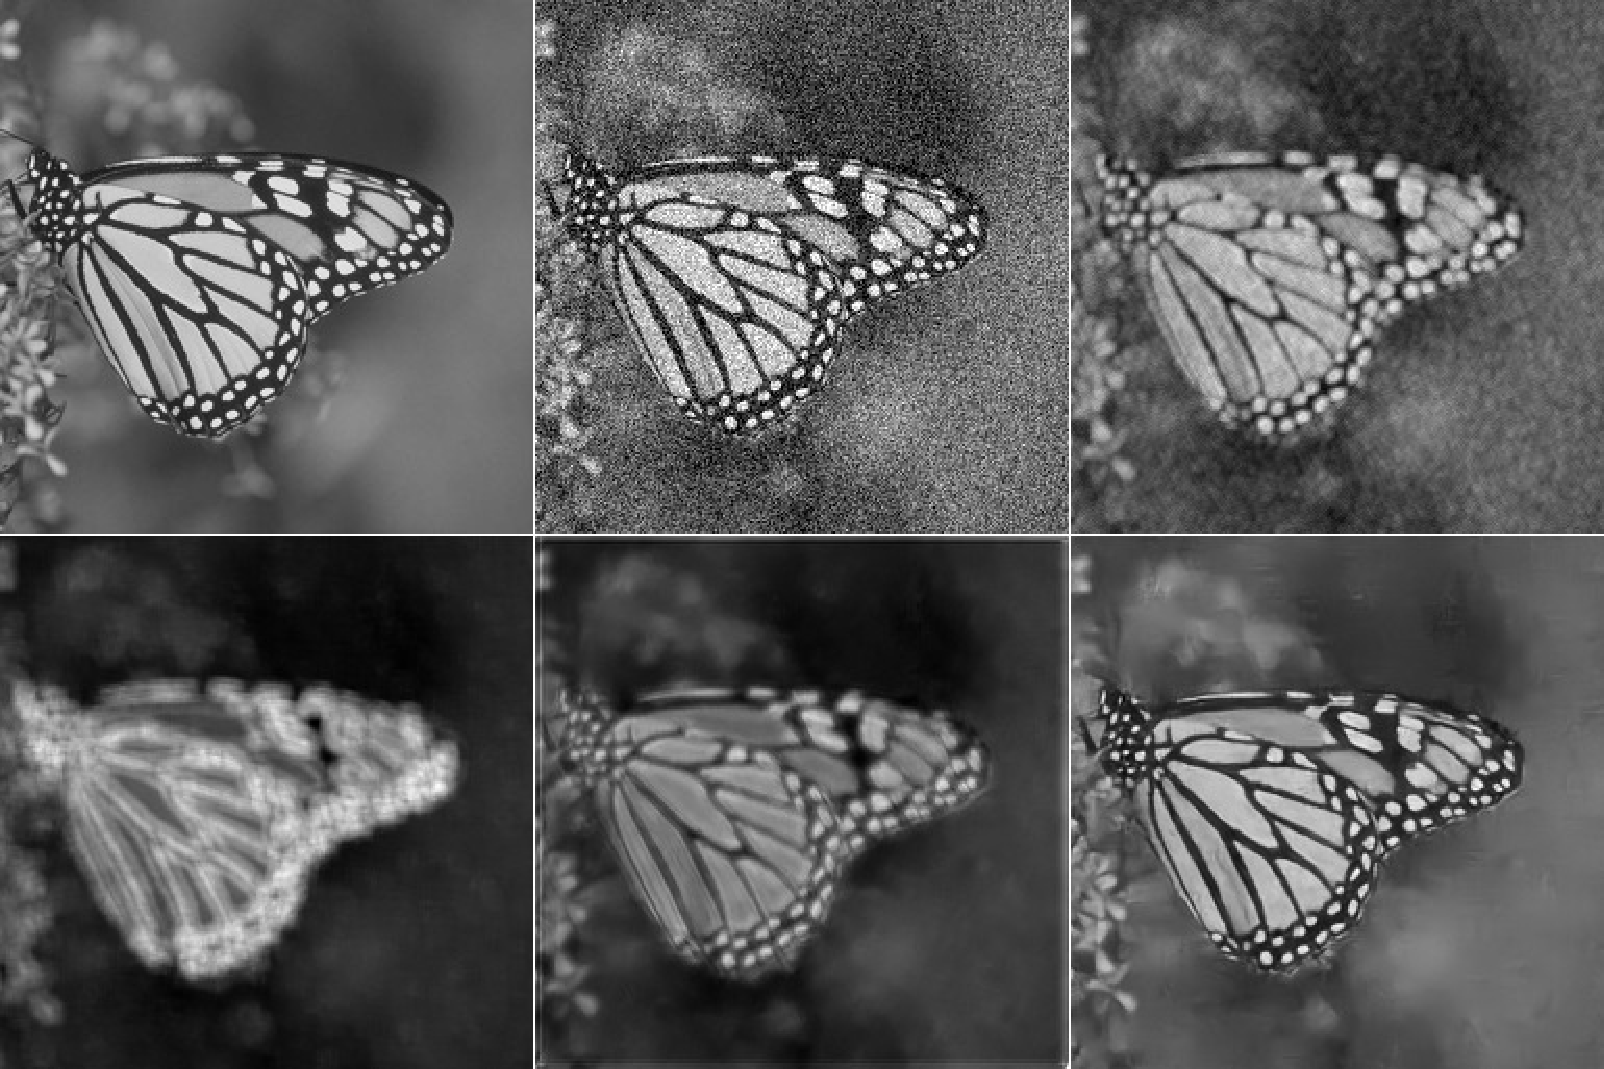
\includegraphics[width=0.48\textwidth]{show-denoising-decv} }
\caption{ (a) Visualization of the 10-layer fully convolutional network. The images from
top-left to bottom-right are: clean image, noisy image, output of conv-2, output of conv-5,
output of conv-8 and output of conv-10, where ``conv-$i$" stands for the $i$-th convolutional layer;
(b) Visualization of the 10-layer convolutional and deconvolutional network. The images from
top-left to bottom-right are: clean image, noisy image, output of conv-2, output of conv-5,
output of deconv-3 and output of deconv-5, where ``deconv-$i$" stands for the $i$-th deconvolutional layer.}
\label{fig3}
\end{figure}




\subsection{Skip connections}

An intuitive question is that, is a network with deconvolution able to recover image details from
the image abstraction only? We find that in shallow networks with only a few layers
of convolution layers, deconvolution is able to recover the details. However, when the
network goes deeper or using operations such as max pooling, even with deconvolution layers, it does not work
that well, possibly because too much details are already lost in the convolution and pooling.


The second question is that, when our network goes deeper, does it achieve performance gain?
We observe that deeper networks in image restoration tasks tend to easily suffer from
performance degradation. The reason may be two folds. First of all, with more layers of
convolution, a significant amount of image details could be lost or corrupted. Given only the image abstraction,
recovering its details is an under-determined problem. Secondly, in terms of optimization,
deep networks often suffer from gradients vanishing and become much harder to train---a problem
that is well addressed in the literature of neural networks.


To address the above two problems, inspired by highway networks \cite{DBLP:journals/corr/SrivastavaGS15}
and deep residual networks \cite{DBLP:journals/corr/HeZRS15}, we add skip connections between
two corresponding convolutional and deconvolutional layers as shown in Figure \ref{fig1}.
A building block is shown in Figure \ref{fig4}. There are two reasons for using such connections.
First, when the network goes deeper, as mentioned above, image details can be lost, making deconvolution
weaker in recovering them. However, the feature maps passed by skip connections carry much image detail,
which helps deconvolution to recover an improved clean version of the image. Second, the skip connections also achieve
benefits on back-propagating the gradient to bottom layers, which makes training deeper network much
easier as observed in \cite{DBLP:journals/corr/SrivastavaGS15} and \cite{DBLP:journals/corr/HeZRS15}.

Note that our skip layer connections are very different from the ones proposed in
\cite{DBLP:journals/corr/SrivastavaGS15} and \cite{DBLP:journals/corr/HeZRS15}, where the only concern
is on the optimization side. In our case, we want to pass information of the convolutional feature maps
to the corresponding deconvolutional layers. The very deep highway networks
\cite{DBLP:journals/corr/SrivastavaGS15} are essentially feedforward long short-term memory (LSTMs)
with forget gates, and the CNN layers of deep residual network \cite{DBLP:journals/corr/HeZRS15}
are feedforward LSTMs without gates. Note that our networks are in general not in the format of
standard feedforward LSTMs.

\begin{figure}[htb!]
\centering
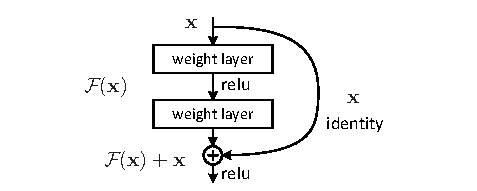
\includegraphics[width=0.48\textwidth]{block}
\caption{An example of a building block in the proposed framework. The rectangle in solid and
dotted lines denote convolution and deconvolution respectively. $\oplus$ denotes element-wise sum of feature maps.}
\label{fig4}
\end{figure}

Instead of directly learning the mappings from the input $X$ to the output $Y$, we would like the network
to fit the residual~\cite{DBLP:journals/corr/HeZRS15} of the problem, which is denoted as $\mathcal{F}(X)=Y-X$.
Such a learning strategy is applied to inner blocks of the encoding-decoding network to make training more
effective. Skip connections are passed every two convolutional layers to their mirrored deconvolutional
layers. Other configurations are possible and our experiments show that this configuration already works
very well. Using such shortcuts makes the network easier to be trained and gains restoration performance
by increasing the network depth.




\subsection{Training}

In general, there are three types of layers in our network: convolution, deconvolution
and element-wise sum. Each layer is followed by a Rectified Linear Unit (ReLU)
~\cite{DBLP:conf/icml/NairH10}. Let $X$ be the input, the convolutional and
deconvolutional layers are expressed as:
\begin{equation}
F(X) = \max(0,W_k * X + B_k),
\end{equation}
where $W_k$ and $B_k$ represent the filters and biases, and $*$ denotes either
convolution or deconvolution operation for the convenience of formulation.
For element-wise sum layer, the output is the element-wise sum of two inputs
of the same size, followed by the ReLU activation:
\begin{equation}
F(X_1,X_2) = \max(0, X_1 + X_2)
\end{equation}

Learning the end-to-end mapping from corrupted images to clean images needs to
estimate the weights $\Theta$ represented by the convolutional and deconvolutional
kernels. Specifically, given a collection of $N$ training sample pairs $\{X^i,Y^i\}$,
where $X^i$ is a noisy image and $Y^i$ is the clean version as the groundtruth.
We minimize the following Mean Squared Error (MSE):
\begin{equation}
  \mathcal{L}(\Theta) = \frac{1}{N}\sum_{i=1}^{N}\|\mathcal{F}(X^i;\Theta)-Y^i\|_F^2.
\label{eq1}
\end{equation}

Traditionally, a  network can learn the mapping from the corrupted image to the clean version
directly. However, our network learns for the additive corruption from the input since there
is a skip connection between the input and the output of the network.
%
%
%
We found that optimizing for the corruption converges better than
optimizing for the clean image. In the extreme case, if the input is a clean image, it would be easier
to push the network to be zero mapping (learning the corruption) than to fit an identity
mapping (learning the clean image) with a stack of nonlinear layers.

We implement and train our network using Caffe~\cite{jia2014caffe}. Empirically, we find
that using Adam~\cite{DBLP:journals/corr/KingmaB14} with base learning rate of $10^{-4}$ for
training converges faster than traditional stochastic gradient descent (SGD). The base
learning rate for all layers are the same, different from ~\cite{DBLP:journals/pami/DongLHT16,
DBLP:conf/nips/JainS08}, in which a smaller learning rate is set for the last layer.
This  is not necessary in our network. Specifically, gradients with respect to the
parameters of $i$th layer is firstly computed as:
\begin{equation}
g = \nabla_{\theta_i}\mathcal{L}(\theta_i).
\end{equation}
Then, the two momentum vectors are computed as:
\begin{equation}
m = \beta_1m + (1 - \beta_1)g,\quad v = \beta_2v + (1-\beta_2)g^2.
\end{equation}
The update rule is:
\begin{equation}
\alpha = \alpha\sqrt{1-\beta_2^t}/(1-\beta_1^t), \quad \theta_i=\theta_i-\alpha m/(\sqrt{v}+\epsilon).
\end{equation}
$\beta_1$, $\beta_2$ and $\epsilon$ are set as the recommended values in~\cite{DBLP:journals/corr/KingmaB14}.

300 images from the Berkeley Segmentation Dataset (BSD)~\cite{MartinFTM01} are used to
generate image patches as the training set for each image restoration task.
%
%
%




\subsection{Testing}

Although trained on local patches, our network can perform restoration on images of arbitrary sizes.
Given a testing image, one can simply go forward through the network, which is already able to
 outperform existing methods. To achieve even better results, we propose
to process a corrupted image on multiple orientations. Different from segmentation, the
filter kernels in our network only eliminate the corruptions, which is usually not sensitive
to the orientation of image contents in low level restoration tasks. Therefore, we can rotate
and mirror flip the kernels and perform forward multiple times, and then average the output to
achieve an ensemble of multiple tests. We see that this can lead to slightly better performance.


\section{Evaluation}
In this section, we present a comparative performance evaluation of our proposed method.
Specifically, we conduct experiments on the widely-used fine-grained benchmark Caltech-UCSD birds dataset \cite{DatasetCUB200} (CUB200-2011).
The classification task is to discriminate among 200 species of birds, and is challenging for computer vision systems due to the high degree of similarity between categories.
It contains 11,788 images of 200 bird species. Each image is annotated with its bounding box and the image coordinates of fifteen keypoints: the beak, back, breast, belly, forehead, crown, left eye, left leg, left wing, right eye, right leg, right wing, tail, nape and throat. We train and test on the splits included with the dataset, which contain around 30 training samples for each species.
Following the protocol of \cite{dpd}, we use two semantic parts for the bird dataset: head and body.
%Figure~\ref{fig:ningfig} (left) illustrates the set of keypoints which comprise the head part, and Figure~\ref{fig:ningfig} (right) illustrates the body part.

We use the open-source package Caffe~\cite{Jia13caffe} to extract deep features and fine-tune our CNNs. For object and part detections, we use the Caffe reference model, which is almost identical to the model used by Krizhevsky et al. in \cite{krizhevsky}. We refer deep features from each layer as \texttt{conv}$n$, \texttt{pool}$n$, or \texttt{fc}$n$ for the $n$th layer of the CNN, which is the output of a convolutional,
pooling, or fully connected layer respectively.
We use \texttt{fc6} to train R-CNN object and part detectors as well as image representation for classification.
%We use \texttt{fc6} to train R-CNN object and part detectors as well as image representation for classification, except in the experiments using fine-tuned networks where \texttt{fc7} features are used, as these features are directly optimized for input into a linear classifier on the target bird classification task.
For $\delta^{NP}$, nearest neighbors are computed using \texttt{pool5}  and cosine distance metric.


\subsection{Fine-grained categorization}
We first present results on the standard fine-grained categorization task associated with the Caltech-UCSD birds dataset.
The first set of results in Table~\ref{tab:finegrainedres} are achieved in the setting where the ground truth bounding box for the entire bird is known at test time, as most state-of-art methods assume, making the categorization task somewhat easier. 
In this setting, our part-based method with the local non-parametric geometric constraint $\delta^{NP}$ works the best without fine-tuning, achieving 68.1\% classification accuracy without fine-tuning.
Fine-tuning improves this result by a large margin, to over 76\%.
We compare our results against three state-of-the-art baseline approaches with results assuming the ground truth bounding box at test time. We use deep convolutional features as the authors of \cite{decaf}, but they use a HOG-based DPM as their part localization method. The increase in performance is likely due to better part localization (see Table \ref{tab:partlocalres}). Oracle method uses the ground truth bounding box and part annotations for both training and test time. 

The second set of results is in the less artificial setting where the bird bounding box is \emph{unknown} at test time. Most of the literature on this dataset doesn't  report performance in this more difficult, but more realistic setting. As Table \ref{tab:finegrainedres} shows, in this setting our part-based method works much better than the baseline DPD model. We achieve 66.0\% classification accuracy without finetuning , almost as good as the accuracy we can achieve when the ground truth bounding box is given. This means there is no need to annotate any box during test time to classify the bird species. With finetuned CNN models, our method achieves 73.89\% classification accuracy. 
We are unaware of any other published results in this more difficult setting, but we note that our method outperforms previous state-of-the-art even without knowledge of the ground truth bounding box.

Another interesting experiment we did is to remove the part descriptors by only looking at the image descriptors inside the predicted bounding box. By having geometric constraints over part locations relative to object location, our method is able to help localize the object. As Table \ref{tab:finegrained_noparts} shows, our method outperforms a single object detector using R-CNN, which means the geometric constraints helps our method better localize the object window. The detection of strong DPM is not as accurate as our method, which explains the performance drop.
The ``oracle'' method uses the ground truth bounding box and achieves 57.94\% accuracy, which is still much lower than the method in Table \ref{tab:finegrainedres} of using both image descriptors inside object and parts.


\begin{table}[t]
\centering
\caption{Fine-grained categorization results on CUB200-2011 bird dataset. -ft means extracting deep features from finetuned CNN models using each semantic part. Oracle method uses the ground truth bounding box and part annotations for both training and test time. } 
\begin{tabular}{|l|r|}
\hline
\multicolumn{2}{|c|}{Bounding Box Given} \\
\hline
DPD~\cite{dpd} & 50.98\% \\
DPD+DeCAF feature ~\cite{decaf} & 64.96\% \\
POOF~\cite{poof} & 56.78\% \\
Symbiotic Segmentation~\cite{iccv13_symbiotic} & 59.40\% \\
Alignment~\cite{iccv13_alignment} & 62.70\%\\
\hline
Oracle & 72.83\% \\
Oracle-ft & 82.02\%\\
\hline
Ours ($\Delta_{\mathrm{box}}$) & 67.55\% \\
Ours ($\Delta_{\mathrm{geometric}}$ with $\delta^{MG}$) & 67.98\% \\
Ours ($\Delta_{\mathrm{geometric}}$ with $\delta^{NP}$) & 68.07\% \\
Ours-ft ($\Delta_{\mathrm{box}}$) & 75.34\% \\
Ours-ft ($\Delta_{\mathrm{geometric}}$ with $\delta^{MG}$) &  \textbf{76.37\%}\\
Ours-ft ($\Delta_{\mathrm{geometric}}$ with $\delta^{NP}$) & 76.34\%\\
\hline
\hline
\multicolumn{2}{|c|}{Bounding Box Unknown} \\
\hline
DPD+DeCAF~\cite{decaf} with no bounding box & 44.94\% \\
Ours ($\Delta_{\mathrm{null}}$) & 64.57\% \\
Ours ($\Delta_{\mathrm{box}}$)& 65.22\% \\
Ours ($\Delta_{\mathrm{geometric}}$ with $\delta^{MG}$) &65.98\% \\
Ours ($\Delta_{\mathrm{geometric}}$ with $\delta^{NP}$) & 65.96\% \\
Ours-ft ($\Delta_{\mathrm{box}}$)& 72.73\% \\
Ours-ft ($\Delta_{\mathrm{geometric}}$ with $\delta^{MG}$) & 72.95\% \\
Ours-ft ($\Delta_{\mathrm{geometric}}$ with $\delta^{NP}$) & \textbf{73.89\%} \\
\hline
\end{tabular}
\label{tab:finegrainedres}
\end{table}

\begin{table}[t]
\centering
\caption{Fine-grained categorization results on CUB200-2011 bird dataset with \emph{no parts}. We trained a linear SVM using deep features on all the methods. Therefore only the bounding box prediction is the factor of difference. -ft is the result of extracting deep features from fine-tuned CNN model on bounding box patches. } \label{tab:finegrained_noparts}
\begin{tabular}{|l|r|}
\hline
Oracle (ground truth bounding box) & 57.94\%\\
Oracle-ft & 68.29\% \\
\hline 
Strong DPM \cite{Hossein_ECCV12} & 38.02\% \\
R-CNN~\cite{rcnn} & 51.05\% \\
\hline \hline
Ours ($\Delta_{\mathrm{box}}$)  & 50.17\% \\
Ours ($\Delta_{\mathrm{geometric}}$ with $\delta^{MG}$) & 51.83\% \\
Ours ($\Delta_{\mathrm{geometric}}$ with $\delta^{NP}$) & 52.38\%\\
Ours-ft ($\Delta_{\mathrm{box}}$)  &  62.13\%\\
Ours-ft ($\Delta_{\mathrm{geometric}}$ with $\delta^{MG}$) & 62.06\% \\
Ours-ft ($\Delta_{\mathrm{geometric}}$ with $\delta^{NP}$) & \textbf{62.75\%} \\
\hline
\end{tabular}
\end{table}

\subsection{Part localization}
We now present results evaluating in isolation the ability of our system to accurately localize parts.
Our results in Table~\ref{tab:partlocalres} are given in terms of the Percentage of Correctly Localized Parts (PCP) metric. 
For the first set of results, the whole object bounding box is given and the task is simply to correctly localize the parts inside of this bounding box, with parts having $\ge 0.5$ overlap with ground truth counted as correct.

For the second set of results, the PCP metric is computed on top-ranked parts predictions using the objective function described in Sec. 3.2.
Note that in this more realistic setting we do not assume knowledge of the ground truth bounding box at test time -- despite this limitation, our system produces accurate part localizations.
% It is worthy to note that we don't have any assumption that the object bounding box prediction having at least 0.5 overlap with the ground truth bounding box, as some other methods suggested.
% The main point is to show without any knowledge of bounding box at test time, our system is able to produce accurate part localizations. 

\begin{table}[t]
\centering
\caption{Recall of region proposals produced by selective search methods on CUB200-2011 bird dataset. We use ground truth part annotations to compute the recall, as defined by the proportion of ground truth boxes for which there exists a region proposal with overlap at least 0.5, 0.6 and 0.7 respectively.}\label{tab:selective_search_recall}
\begin{tabular}{|c|c|c|c|}
\hline
%\multicolumn{4}{|c|}{Bounding Box Given} \\
%\hline
%Overlap & 0.50 & 0.60 & 0.70\\
%\hline
%Head & 94.71\% &  & \\
%Body & 97.39\%  & & \\
%\hline
%\multicolumn{4}{|c|}{Bounding Box Unknown} \\
%\hline
Overlap & 0.50 & 0.60 & 0.70\\
\hline
Bounding box & 96.70\% & 97.68\% & 89.50\% \\
Head &  93.34\% & 73.87\%& 37.57\%\\
Body & 96.70\% & 85.97\%&54.68\%\\
\hline
\end{tabular}
\end{table}

\begin{table}[t]
\centering
\caption{Part localization accuracy in terms of PCP (Percentage of Correctly Localized Parts) on the CUB200-2011 bird dataset. There are two different settings: with given bounding box and without bounding box. } 
\label{tab:partlocalres}
\begin{tabular}{|l|r|r|}
\hline
\multicolumn{3}{|c|}{Bounding Box Given} \\
\hline
& \multicolumn{1}{|c|}{Head}
& \multicolumn{1}{|c|}{Body}
\\
\hline
Strong DPM~\cite{Hossein_ECCV12} & 43.49\% & 75.15\% \\
Ours ($\Delta_{\mathrm{box}}$)   & 61.40\% & 65.42\% \\
Ours ($\Delta_{\mathrm{geometric}}$ with $\delta^{MG}$)& 66.03\% & 76.62\% \\
Ours ($\Delta_{\mathrm{geometric}}$ with $\delta^{NP}$) & \textbf{68.19\%} & \textbf{79.82\%} \\
\hline
\multicolumn{3}{|c|}{Bounding Box Unknown} \\
\hline
& \multicolumn{1}{|c|}{Head}
& \multicolumn{1}{|c|}{Body}
\\
\hline
Strong DPM~\cite{Hossein_ECCV12} & 37.44\% & 47.08\% \\
Ours ($\Delta_{\mathrm{null}}$  ) &60.50\% &  64.43\% \\
Ours ($\Delta_{\mathrm{box}}$)  & 60.56\% & 65.31\% \\
Ours ($\Delta_{\mathrm{geometric}}$ with $\delta^{MG}$)& \textbf{61.94\%} & 70.16\% \\ 
Ours ($\Delta_{\mathrm{geometric}}$ with $\delta^{NP}$) & 61.42\% & \textbf{70.68\%} \\
\hline
\end{tabular}
\end{table}

\begin{figure*}[t]
\begin{center}
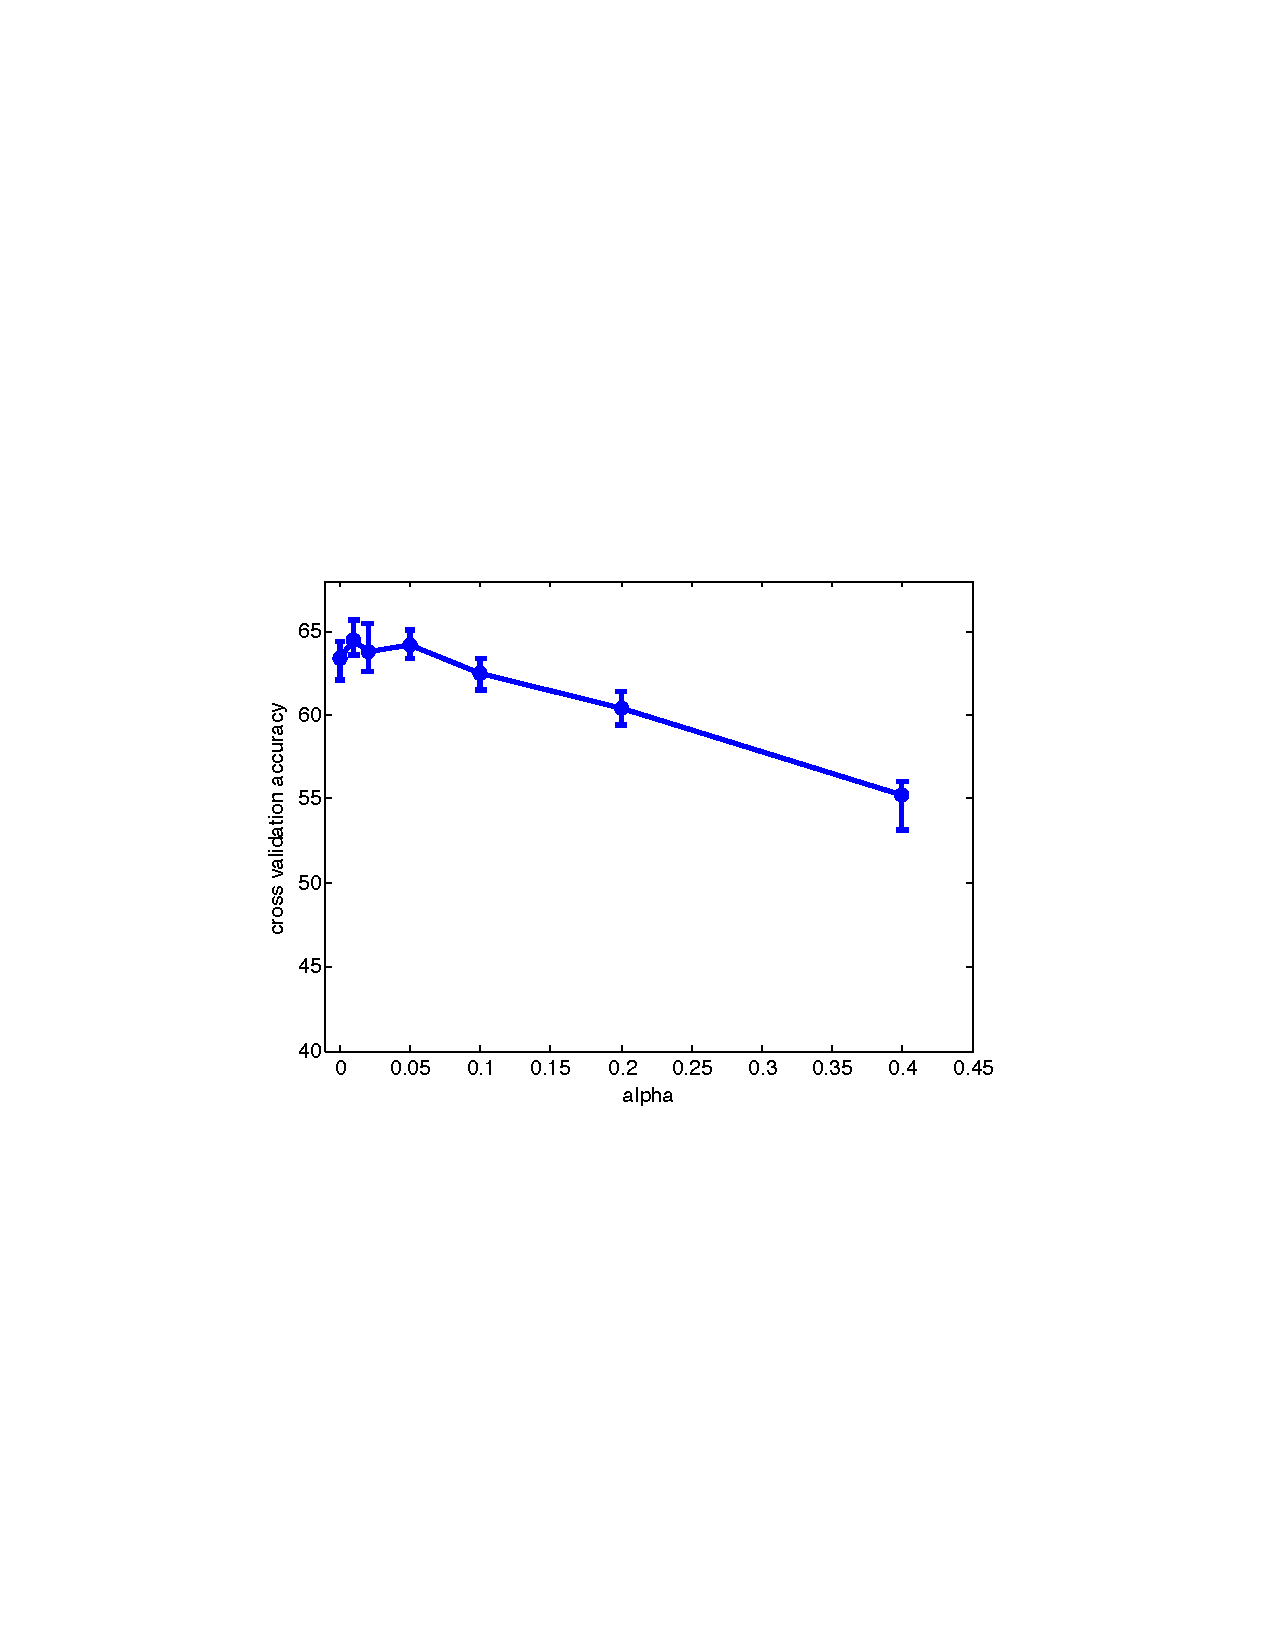
\includegraphics[width=0.45\linewidth]{alpha_plot.pdf}
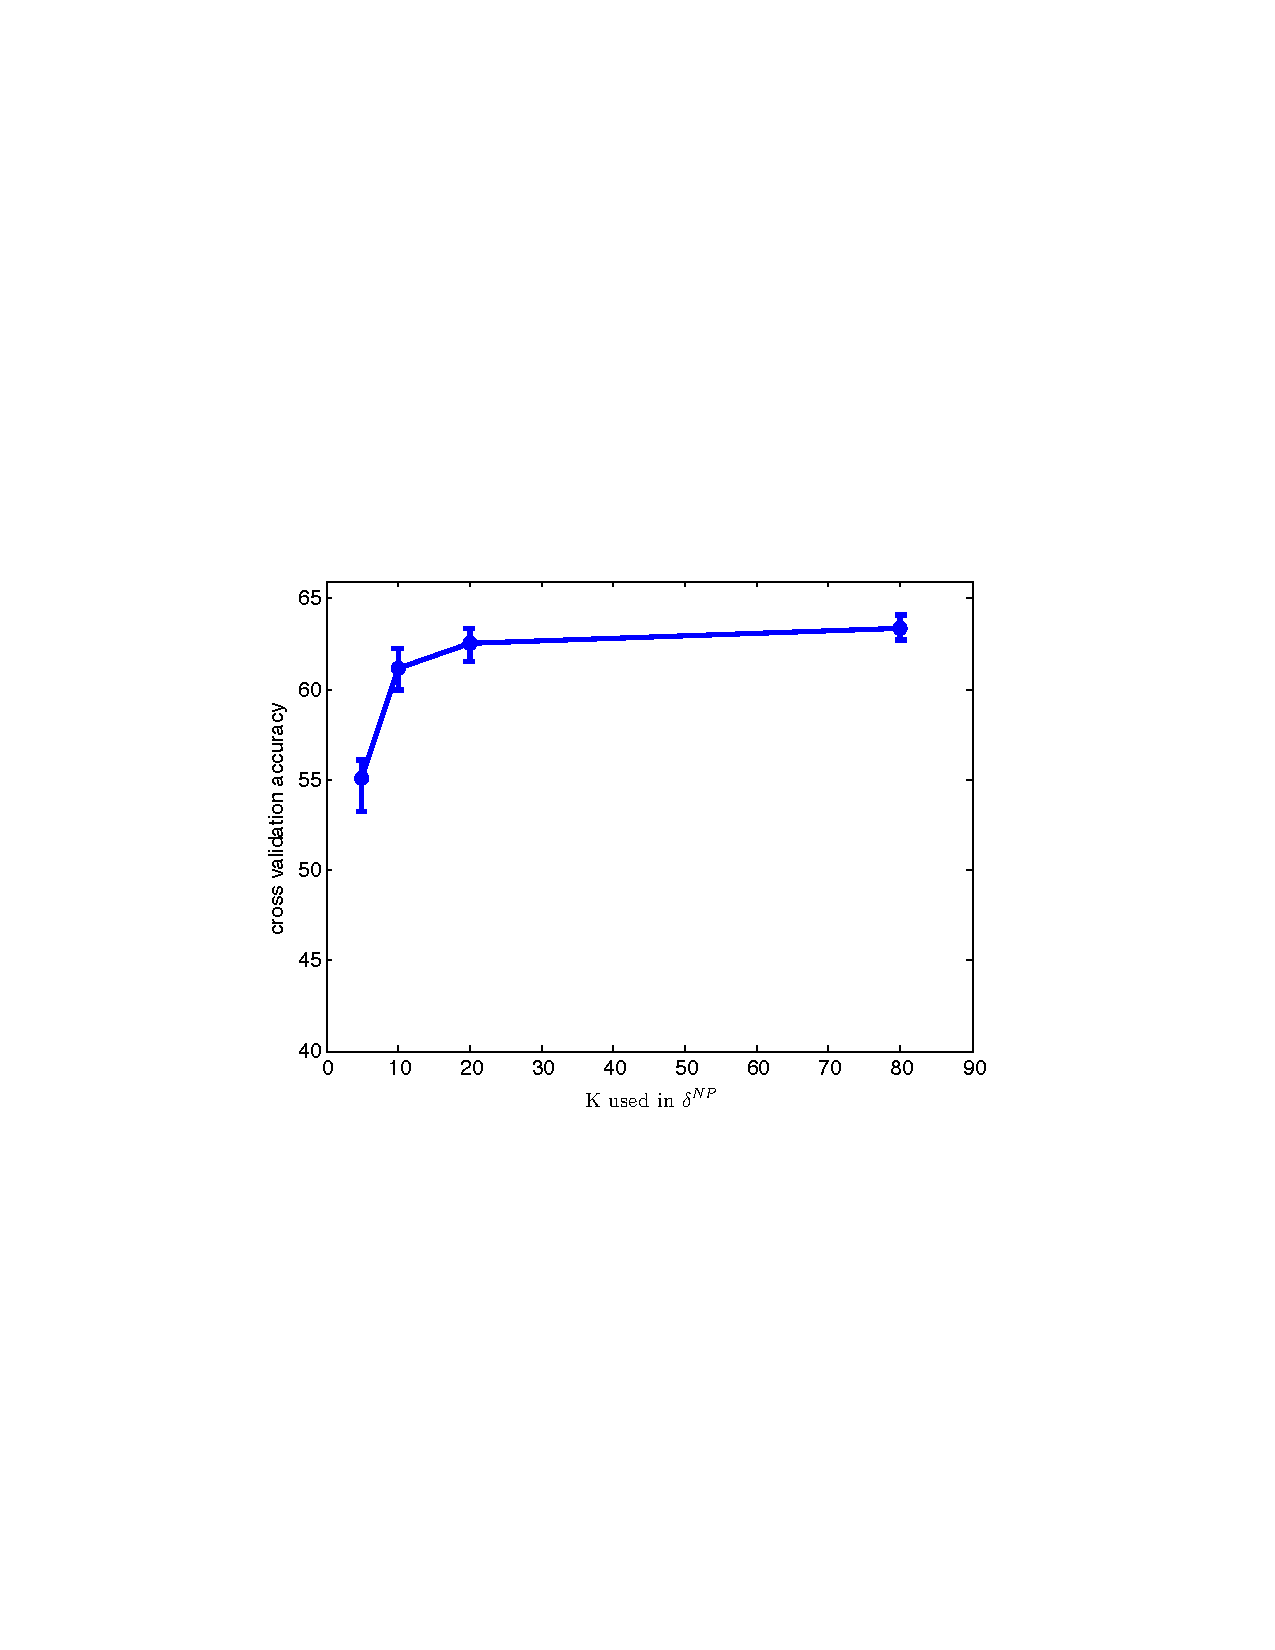
\includegraphics[width=0.45\linewidth]{K_plot.pdf}
\end{center}
\caption{Cross-validation results on fine-grained accuracy for different values of $\alpha$ (left) and $K$ (right). We split the training data into 5 folds and use cross-validate each hyperparameter setting.}
\label{fig:crossvalidationalphak}
\end{figure*}




As shown in Table \ref{tab:partlocalres}, for both settings of given bounding box and unknown bounding box, our methods outperform the strong DPM~\cite{Hossein_ECCV12} method.
Adding a geometric constraint $\delta^{NP}$ improves our results (79.82\% for body localization compared to 65.42\%). In the fully automatic setting, the top ranked detection and part localization performance on head is 65\% better than the baseline method. $\Delta_{\mathrm{null}}=1$ is the appearance-only case with no geometric constraints applied. Although the fine-grained classification results don't show a big gap between $\Delta_{\mathrm{geometric}}$ and $\Delta_{\mathrm{box}}$, we can see the performance gap for part localization.
The reason for the small performance gap might be that deep convolutional features are invariant to small translations and rotations,
limiting the impact of small localization errors on our end-to-end accuracy.


We also evaluate the recall performance of selective search region proposals \cite{selsearch} for bounding box and semantic parts. 
The results of recall given different overlapping thresholds are shown in Table \ref{tab:selective_search_recall}. 
Recall for the bird head and body parts is high when the overlap requirement is $0.5$, which provides the foundation for localizing these parts given the region proposals. However, we also observe that the recall for head is below $40\%$ when the overlap threshold is $0.7$, indicating the bottom-up region proposals could be a bottleneck for precise part localization.

Other visualizations are shown in Figure~\ref{fig:comparasion}. We show three detection and part localization for each image, the first column is the output from strong DPM, the second column is our methods with individual part predictions and the last column is our method with local prior. We used the model pretrained from \cite{Hossein_ECCV12} to get the results. We also show some failure cases of our method in Figure~\ref{fig:failure}.


\subsection{Component Analysis}
To examine the effect of different values of $\alpha$ and $K$ used in $\Delta_{\mathrm{geometric}}$, we conduct cross-validation experiments.
Results are shown in Figure~\ref{fig:crossvalidationalphak}. We fix $K=20$ in Figure~\ref{fig:crossvalidationalphak}, left and fix $\alpha = 0.1$ in Figure \ref{fig:crossvalidationalphak}, right. All the experiments on conducted on training data in a cross-validation fashion and we split the training data into 5 folds.
%\todo{can we add error bars? ... if you still have the results}.
As the results show, the end-to-end fine-grained classification results are sensitive to the choice of $\alpha$ and $\alpha=0$ is the case of $\Delta_{\mathrm{box}}$ predictions without any geometric constraints. The reason why we have to pick a small $\alpha$ is the pdf of the Gaussian is large compared to the logistic score function output from our part detectors. On the other hand, the choice of $K$ cannot be too small and it is not very sensitive when $K$ is larger than 10. 


%Experiment results vary K, vary $\alpha$
%Answer the following questions,
%1) Are parts necessary, show results with only root filter
%2) Are neighbors necssarcy, show only fit into one Gaussian
%3) Show hor prior helps, show results without prior
%
%figure to visualize the prior over neighbors v.s. prior over the whole training data


\begin{figure*}
\begin{center}
\begin{tabular}{ccc}
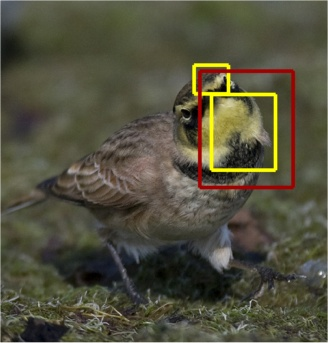
\includegraphics[width=0.3\linewidth]{6_strong_dpm.jpg} &
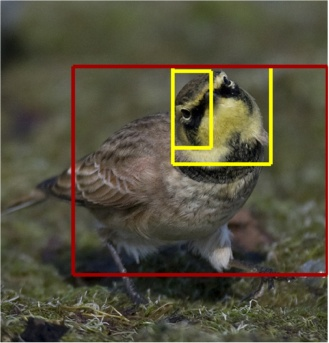
\includegraphics[width=0.3\linewidth]{6_individual.jpg} &
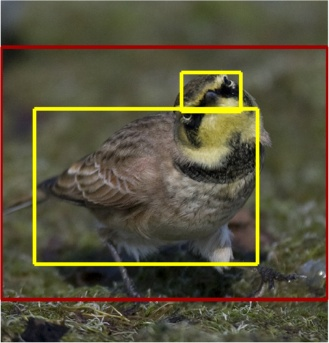
\includegraphics[width=0.3\linewidth]{6_neighbor.jpg} \\
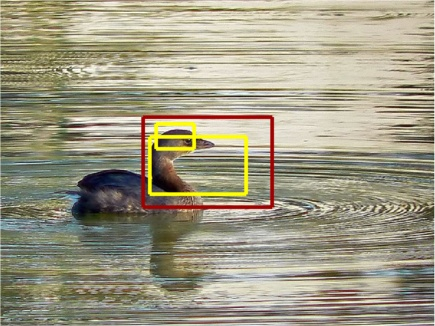
\includegraphics[trim=0mm 10mm 0mm 10mm, clip, width=0.3\linewidth]{11_strong_dpm.jpg} &
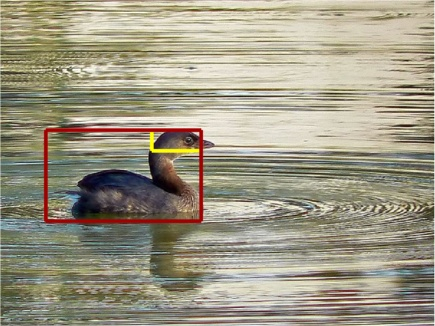
\includegraphics[trim=0mm 10mm 0mm 10mm, clip, width=0.3\linewidth]{11_individual.jpg} &
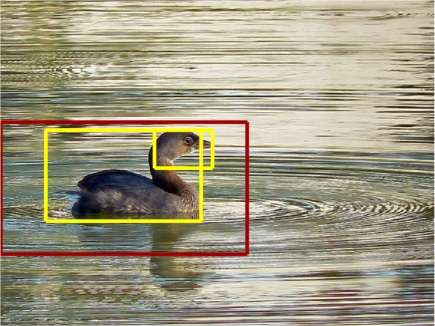
\includegraphics[trim=0mm 10mm 0mm 10mm, clip, width=0.3\linewidth]{11_neighbor.jpg} \\
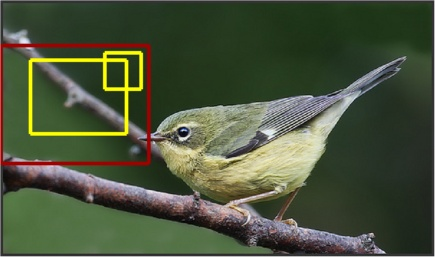
\includegraphics[width=0.3\linewidth]{13_strong_dpm.jpg} &
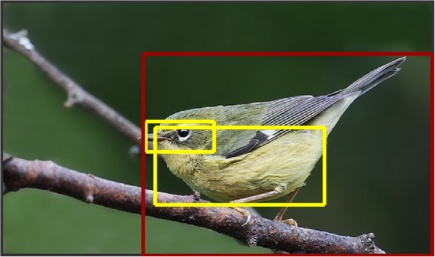
\includegraphics[width=0.3\linewidth]{13_individual.jpg} &
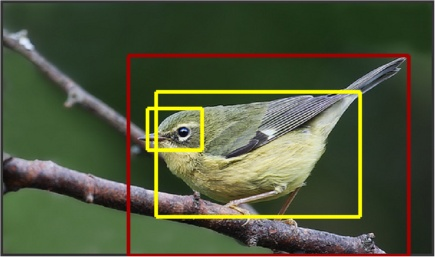
\includegraphics[width=0.3\linewidth]{13_neighbor.jpg} \\
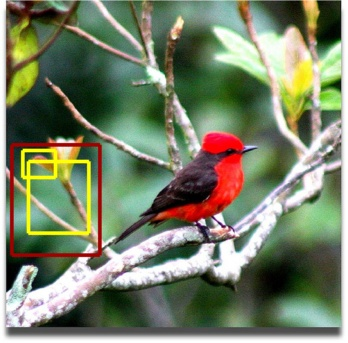
\includegraphics[trim=0mm 20mm 0mm 20mm, clip, width=0.3\linewidth]{15_strong_dpm.jpg} &
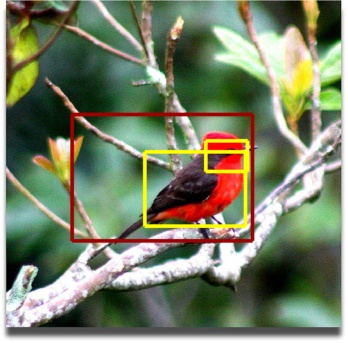
\includegraphics[trim=0mm 20mm 0mm 20mm, clip, width=0.3\linewidth]{15_individual.jpg} &
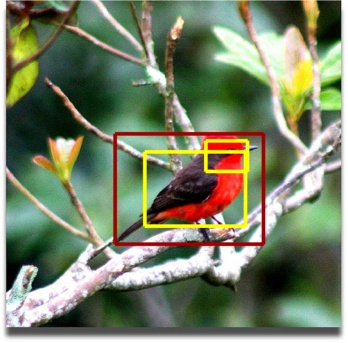
\includegraphics[trim=0mm 20mm 0mm 20mm, clip, width=0.3\linewidth]{15_neighbor.jpg} \\
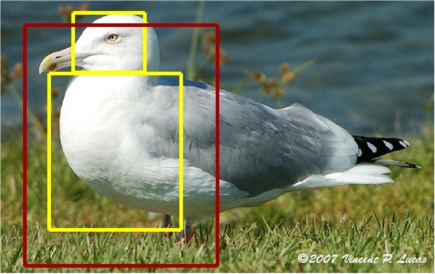
\includegraphics[width=0.3\linewidth]{16_strong_dpm.jpg} &
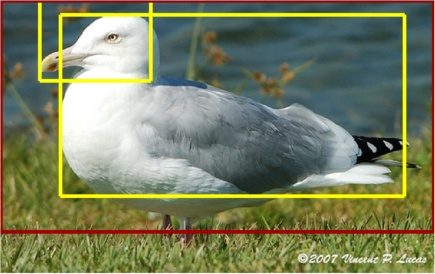
\includegraphics[width=0.3\linewidth]{16_individual.jpg} &
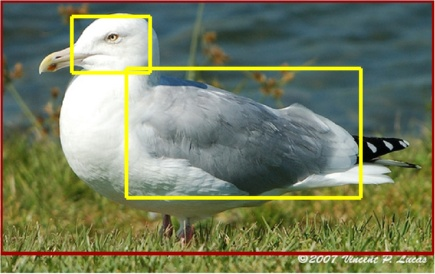
\includegraphics[width=0.3\linewidth]{16_neighbor.jpg} \\
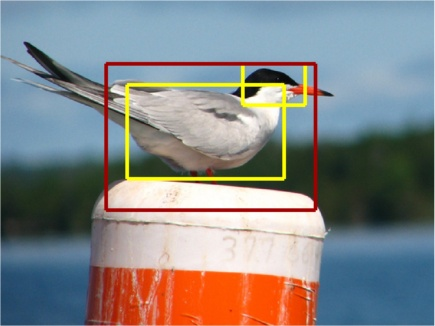
\includegraphics[width=0.3\linewidth]{17_strong_dpm.jpg} &
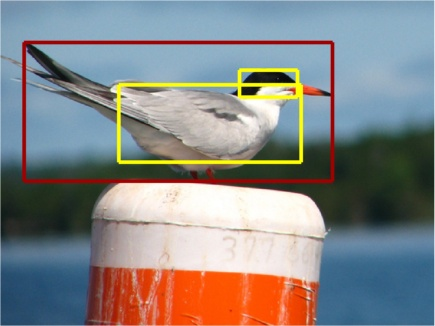
\includegraphics[width=0.3\linewidth]{17_individual.jpg} &
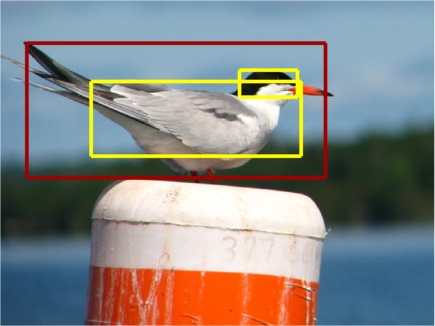
\includegraphics[width=0.3\linewidth]{17_neighbor.jpg} \\
% 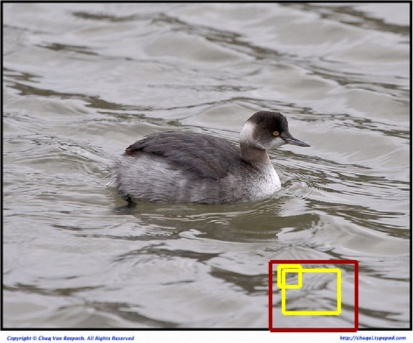
\includegraphics[width=0.3\linewidth]{19_strong_dpm.jpg} &
% 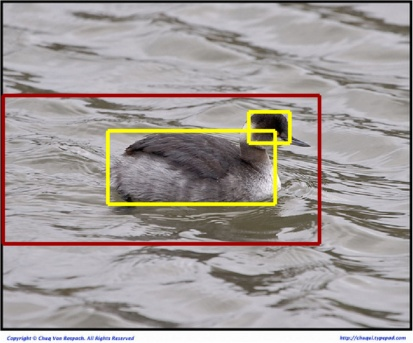
\includegraphics[width=0.3\linewidth]{19_individual.jpg} &
% 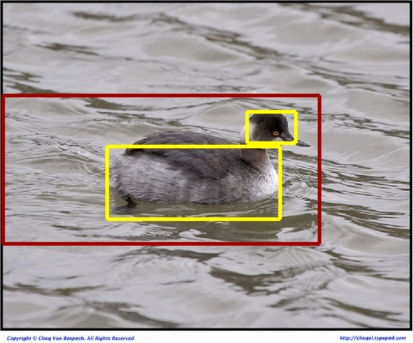
\includegraphics[width=0.3\linewidth]{19_neighbor.jpg} \\
% 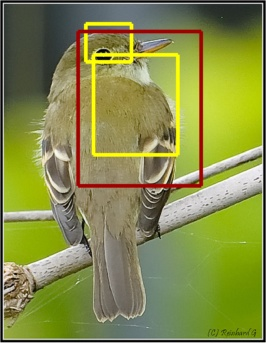
\includegraphics[width=0.3\linewidth]{30_strong_dpm.jpg} &
% 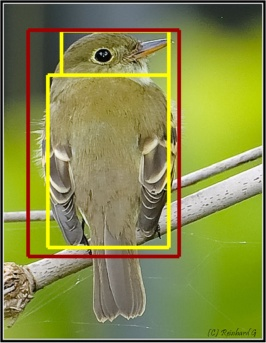
\includegraphics[width=0.3\linewidth]{30_individual.jpg} &
% 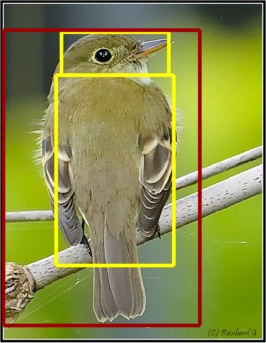
\includegraphics[width=0.3\linewidth]{30_neighbor.jpg} \\
Strong DPM & Ours ($\Delta_{box}$) & Ours ($\delta^{NP}$)
\\
\end{tabular}
\end{center}
\caption{{Examples of bird detection and part localization from strong DPM~\cite{Hossein_ECCV12} (left); our method using $\Delta_{\mathrm{box}}$ part predictions (middle); and our method using $\delta^{NP}$(right). All detection and localization results without any assumption of bounding box. }}
\label{fig:comparasion}
\end{figure*}

\begin{figure*}
\begin{center}
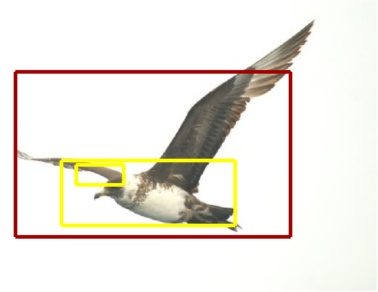
\includegraphics[height=0.2\linewidth]{8_neighbor.jpg} 
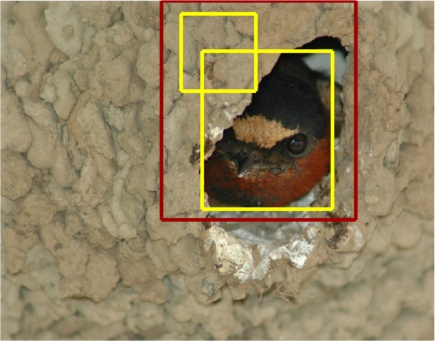
\includegraphics[height=0.2\linewidth]{32_neighbor.jpg} 
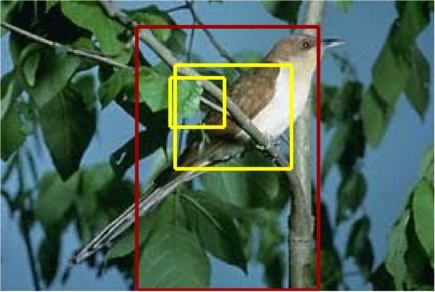
\includegraphics[height=0.2\linewidth]{41_neighbor.jpg} 
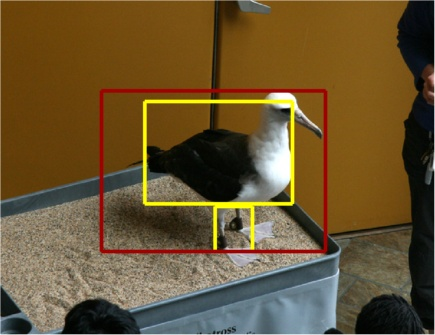
\includegraphics[height=0.2\linewidth]{57_neighbor.jpg} 
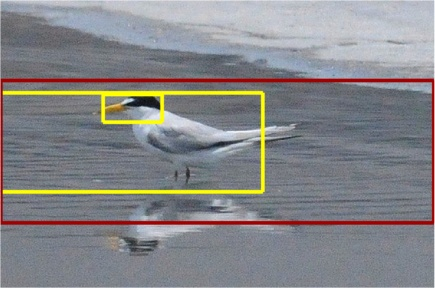
\includegraphics[height=0.2\linewidth]{58_neighbor.jpg}
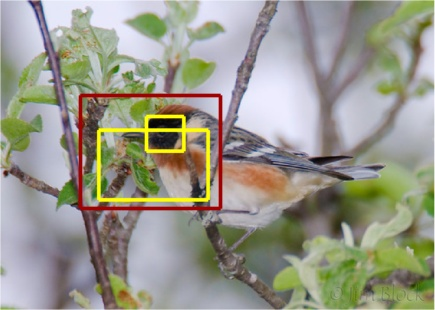
\includegraphics[height=0.2\linewidth]{64_neighbor.jpg} 
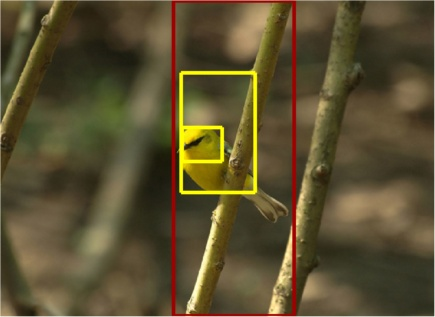
\includegraphics[height=0.2\linewidth]{99_neighbor.jpg} 
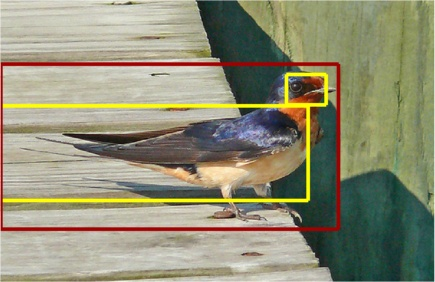
\includegraphics[height=0.2\linewidth]{47_neighbor.jpg} 
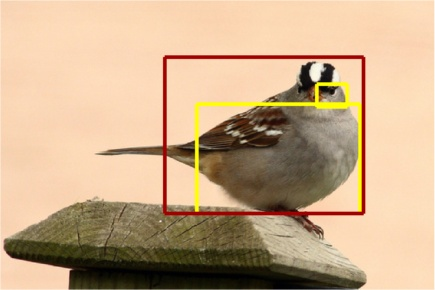
\includegraphics[height=0.2\linewidth]{91_neighbor.jpg} 
\end{center}
\caption{{Failure cases of our part localization using $\delta^{NP}$.}}
\label{fig:failure}
\end{figure*}


\label{sec:conclusion}
We introduce a novel neural network architecture, the Synchronized Spectral CNN (SyncSpecCNN), for semantic annotation on 3D shape graphs. To share coefficients and conduct multi-scale analysis in different parts of a single shape graph, we introduce a spectral parametrization of dilated convolutional kernels. To allow parameter sharing across related but different shapes that may be represented by very different graphs, we introduce a spectral transformer network to synchronize different spectral domains. The effectiveness of different components in our network is validated through extensive experiments. Jointly these contributions lead to state-of-the-art performance on various semantic annotation tasks including 3D shape part segmentation and 3D keypoint prediction.

\newpage
\bibliographystyle{splncs03}
\bibliography{reference}
\end{document}
